% \iffalse meta-comment
%<=*COPYRIGHT>
%% Copyright (C) 2006-2012 by Martin Scharrer <martin@scharrer-online.de>
%% -----------------------------------------------------------------------
%% This work may be distributed and/or modified under the
%% conditions of the LaTeX Project Public License, either version 1.3
%% of this license or (at your option) any later version.
%% The latest version of this license is in
%%   http://www.latex-project.org/lppl.txt
%% and version 1.3 or later is part of all distributions of LaTeX
%% version 2005/12/01 or later.
%%
%% This work has the LPPL maintenance status `maintained'.
%%
%% The Current Maintainer of this work is Martin Scharrer.
%%
%% This work consists of the files svn-multi.dtx and svn-multi.ins
%% and the derived filebase svn-multi.sty and svnkw.sty.
%%
%<=/COPYRIGHT>
% \fi
%
% \iffalse
%<*driver>
\ProvidesFile{svn-multi.dtx}[%
%<=*DATE>
    2011/08/30
%<=/DATE>
%<=*VERSION>
    v2.4d
%<=/VERSION>
    svn-multi DTX file]
\documentclass{ydoc}[2011/03/19]
\GetFileInfo{svn-multi.dtx}
\usepackage[english]{babel}
\dateenglish

\usepackage{svn-multi}[2011/08/30]
\newcommand{\ie}{i.e.\@\xspace}
\newcommand{\eg}{e.g.\@\xspace}

\def\DescribeOption{\par\smallskip\noindent\optpar}
\let\scr\pkg
\def\svnmulti{\pkg{svn-multi}\xspace}
\let\csi\cs
\let\csd\cs

\usepackage{graphicx}

\EnableCrossrefs
%\DisableCrossrefs
\CodelineIndex
%\PageIndex
\RecordChanges
\OnlyDescription
\widowpenalty=500
\clubpenalty=500
\listfiles
\begin{document}
  \DocInput{svn-multi.dtx}%
  \PrintChanges
  %\clearpage
  \PrintIndex
\end{document}
%</driver>
% \fi
%
% \CheckSum{2887}
%
% {\makeatother
% \CharacterTable
%  {Upper-case    \A\B\C\D\E\F\G\H\I\J\K\L\M\N\O\P\Q\R\S\T\U\V\W\X\Y\Z
%   Lower-case    \a\b\c\d\e\f\g\h\i\j\k\l\m\n\o\p\q\r\s\t\u\v\w\x\y\z
%   Digits        \0\1\2\3\4\5\6\7\8\9
%   Exclamation   \!     Double quote  \"     Hash (number) \#
%   Dollar        \$     Percent       \%     Ampersand     \&
%   Acute accent  \'     Left paren    \(     Right paren   \)
%   Asterisk      \*     Plus          \+     Comma         \,
%   Minus         \-     Point         \.     Solidus       \/
%   Colon         \:     Semicolon     \;     Less than     \<
%   Equals        \=     Greater than  \>     Question mark \?
%   Commercial at \@     Left bracket  \[     Backslash     \\
%   Right bracket \]     Circumflex    \^     Underscore    \_
%   Grave accent  \`     Left brace    \{     Vertical bar  \|
%   Right brace   \}     Tilde         \~}
% }
% \changes{v1.0}{2006/05/27}{Initial version}
% \changes{v1.1}{2006/06/08}{Added macros to extract and typeset date/time
% information. Added macros to set and typeset main URL or filename.}
% \changes{v1.2}{2007/06/22}{Renamed package from \texttt{svnkw} to
% \texttt{svn-multi} to match CTAN directory. Wrapper file
% \texttt{svnkw.sty} is provided for backward compatibility.}
% \changes{v1.3}{2007/07/01}{Added verbatim support. Keywords can now contain
% special character like \texttt{\_ \^{} \$ \% \& \textbackslash}. Rewrote
% keyword check macros to work with verbatim code. \texttt{\textbackslash
% nofiles} is now obeyed.}
% \changes{v1.3a}{2007/07/10}{Fixed issue with unwanted spaces generated by
% \cs{svnid}, \cs{svnidlong} and \cs{svnkwsave}, \eg when used in a file which
% is included with \css{input}}
% \changes{v1.3b}{2008/12/03}{Changed the way catcodes are modified to be
% compatible with the french option of the babel package or other packages which
% modify the list of special characters.}
% \changes{v1.4}{2009/02/27}{Added support for timezones with non-zero minute
% part, \eg +0530.}
% \changes{v1.5}{2009/02/28}{Added \css{today}-style macros \cs{svntoday} and
% \cs{svnfiletoday}.}
% \changes{v2.0}{2009/03/23}{New features: keyword groups, external file
% support, auto-include of images, files as subgroups and table of revisions.}
% \changes{v2.1}{2009/03/27}{Added automatic extraction of keywords from 
% Subversion 'entries' file: 'autokw' option}
% \changes{v2.2}{2009/10/19}{Added \css{ifsvnmodified} and 
% \css{ifsvnfilemodified} macros. Some bug fixes.}
% \changes{v2.3}{2010/03/30}{Changed \css{svnidlong} to ignore all comments between verbatim arguments.}
% \changes{v2.3}{2010/07/19}{
%      Fixed `autokw` to work with newer versions (1.6.x) of
%        Subversion where the `format` file is not in the `.svn`
%        directory anymore.
%      Added debug output for `autokw` option.
%      svn entries parser: fixed bugs with empty date and
%        revision values.
%      Fixed problem with `\cs{chapter}` defined as `\cs{relax}` in
%        `\cs{tableofrevisions}`.
%      Fixed unwanted spaces.
%      Changed `\cs{svnidlong}` to allow comments with braces
%        between arguments. This avoids problems with latexdiff.
%      Changed catcodes to normal of reading `.svx` files.
%      Updated code documentation.
%      Updated user documentation.
% }
% \changes{v2.4}{2010/12/08}{
%   Persistent data is now written to the '.aux' file, not to the '.svn' file to save a file handle.
%   The 'fink' package usage got replaced by the 'currfile' and 'filehook' packages.
% }
% \changes{v2.4a}{2011/01/03}{
%   Update for new version of the 'currfile' package.
% }
% \changes{v2.4b}{2011/03/20}{Fix for non-ASCII characters in keywords. Added group check for \cs{svnexternal}.}
% \changes{v2.4c}{2011/04/02}{Fix for modified marker 'M' used in \cs{svnid}.}
% \changes{v2.4d}{2011/08/30}{Fix for \cs{include} files in table-of-revisions.}
%
% ^^A \GetFileInfo{svn-multi.dtx}
%
% \DoNotIndex{\newcommand,\newenvironment,\AtBeginDocument,\AtEndDocument}
% \DoNotIndex{\def,\let,\edef,\xdef,\item,\space,\write,\jobname,\relax,\!}
% \DoNotIndex{\closeout,\csname,\DeclareRobustCommand,\else,\empty,\newwrite}
% \DoNotIndex{\endcsname,\expandafter,\fi,\Hurl,\hyper@normalise,\@ifnextchar}
% \DoNotIndex{\ifnum,\@ifundefined,\ifx,\immediate,\InputIfFileExists,\ }
% \DoNotIndex{\newcount,\noexpand,\openout,\PackageWarning,\@percentchar}
% \DoNotIndex{\@sanitize,\@makeother,\@iwsvn,\%,\_,\&,\^,\$,\#,\ ,\\,\if@filesw}
% \DoNotIndex{\gdef,\begingroup,\endgroup,\catcode}
% \DoNotIndex{\^,\ ,\_,\(,\),\$,\&,\#,\@ampersamchar,\AtEndOfPackage}
% \DoNotIndex{\@backslashchar,\begin,\bgroup,\chapter,\day}
% \DoNotIndex{\DeclareOption,\do,\dospecials,\@dottedtocline,\egroup}
% \DoNotIndex{\end,\ExecuteOptions,\svnmulti@date,\svnmulti@version,\@for}
% \DoNotIndex{\futurelet,\g@addto@macro,\global,\@gobbletwo,\hline}
% \DoNotIndex{\hspace,\if@restonecol,\if@twocolumn,\ignorespaces}
% \DoNotIndex{\makeatletter,\MakeUppercase,\@mkboth,\month,\@namedef}
% \DoNotIndex{\NeedsTeXFormat,\newif,\onecolumn}
% \DoNotIndex{\PackageError,\ProcessOptions}
% \DoNotIndex{\ProvidesPackage,\renewcommand,\RequirePackage}
% \DoNotIndex{\@restonecolfalse,\@restonecoltrue,\section,\strut}
% \DoNotIndex{\tableofcontents,\tableofrevisions,\texttt,\today}
% \DoNotIndex{\twocolumn,\@undefined,\url,\year}
% \DoNotIndex{\textwidth,\the,\string,\raggedright,\providecommand,\small,\toks@}
% \DoNotIndex{\medskipamount,\long,\leftskip,\clearpage,\advance,\addtolength}
% \DoNotIndex{\DeclareBoolOption,\DeclareStringOption,\DeclareVoidOption}
% \DoNotIndex{\ProcessKeyvalOptions,\SetupKeyvalOptions}
% \DoNotIndex{\@firstoftwo,\@secondoftwo,\@gobble}
%
% \GetFileInfo{svn-multi.dtx}
% \author{Martin Scharrer}
% \email{martin@scharrer-online.de}
% \ifdefined\repository
%   \repository{https://bitbucket.org/martin_scharrer/svn-multi}
% \fi
% \maketitle
%
% \section{Introduction}
% This package allows to typeset version control (VC) information provided by 
% Subversion\footnote{Subversion homepage: \url{http://subversion.tigris.org/}} 
% keywords (\eg |$||Id: ... $|) in \LaTeX\ documents which can contain of 
% multiple |.tex| files included using |\include| or |\input|.
% Subversion is a modern version control system designed to replace its 
% predecessor CVS and uses integers as revision numbers.
%
% This package reads the keywords of all files and provides the VC information 
% of of the most recent changed file of the document to the user through a set 
% of macros. This information is written to an auxiliary |.aux| file during the 
% first \LaTeX\ run and read back at the next which introduces the same delay 
% known from the table of contents. The standard \LaTeX{} switch |\nofiles| can 
% be used to suppress the file generation.
%
% In addition to this basic functionality several more features are provided:
% \begin{itemize}
%   \item Macros to typeset the VC information of the current source file.
%   \item Access of all parts of the VC date.
%   \item Formatting of author names or revision numbers.
%   \item Definition of groups and subgroups.
%   \item Including of the VC information of external files.
%   \item Table of Revisions.
% \end{itemize}
%
% \subsection{Scope of Keywords}
% This package provides the Subversion keyword data in several different scopes:
% document-global, file-local and, new with v2.0, by group.
%
% \subsubsection*{Document Global}
% The document global macros, like \cs{svnrev}, return the latest version 
% control information (keyword data) for the whole multi-file document, \ie the 
% information of the latest changed file of the document. To collect, sort and 
% provide this information is the main functionality of this package.
%
% \subsubsection*{Local to Current File}
% There are also file-local macros, \eg \cs{svnfilerev}, which return the 
% version control information of the current file, \ie the file they are used 
% in. It is assumed here that every file using this macros calls first either a 
% \cs{svnid} or \cs{svnidlong} macro or both.  See section~\ref{sec:usage:id} 
% for more details about the id macros.  Please note that the file-local macros 
% technically actually return the \emph{last registered} information from the 
% last \cs{svnid} or \cs{svnidlong}. As long the \opt{filehooks} option (new in 
% v2.0) is not enabled (explicit or implicit) this keyword macros will leak from 
% one file over to the next.  This will cause wrong results if they are used in 
% a file before or without any id macros. With this option the macros will be 
% reset at the beginning of every source file of the document.
%
% \subsubsection*{Groups}
% Version 2.0 introduces the concept of groups. Several files of a multi-file 
% \LaTeX\ document can be grouped together and the latest version control 
% information of all files of a group is provided by macros. This works in the 
% same way as the global macros mentioned above but only with the files in the 
% group. It can also be seen from the other side: the macros are local like the 
% file-local macros mentioned above but for all files of the group, not only the 
% current one.
%
% These groups could also be called \textit{file groups}, \textit{keyword 
% groups} or, like in programming languages, \textit{namespaces}. In this manual 
% they will be reference as simple \textit{groups} most the time. In places 
% where they could be confused with \TeX\ groups (|{ }|, |\begingroup| 
% |\endgroup|), \eg ``in the current group'' or ``group local'', they will be 
% called \textit{keyword groups}.
%
% There is no limitation (besides internal \LaTeX\ resource limits) for the 
% number of different groups. The files of one group do not have to be included 
% in a row but can be included everywhere in the document. The version control 
% information of the current group can be typeset with macros like \cs{svncgrev} 
% (|cg| for \emph{current group}).  Also, a general but less robust macro 
% \cs{svng}\marg{group name}\marg{key} is provided to access others groups by 
% name everywhere in the document. To avoid some macro robustness problems the 
% current group can be changed locally for the output macros using 
% \cs{svnsetcg}\marg{group name}.
%
% See section~\ref{sec:group} for further details and usage instructions on 
% group macros.
%
% \section{Usage}
% The version control information are provided by Subversion keywords which
% first need to be read in by dedicated macros and can then be typeset using
% different macros.
%
% \subsection{Package Options}
% Since v2.0 this package provides options to enable only a needed features, \eg 
% to avoid problems with other packages or save \TeX\ memory. For backwards 
% compatibility to pre-2.0 package versions all old features are enabled by 
% default and all new features are disabled to save a little of \TeX\ memory.
%
% All options except the first two are boolean key=value options (so far) and
% await either `|true|' or `|false|' as value. A missing value means `|true|'.
% So \eg |[groups=true,verbatim=false,external]|, enables the \opt{external} and
% \opt{groups} options but disables the \opt{verbatim} option.
%
% The available options are:\par
%
% \DescribeOption{old}
% Only pre-v2.0 features are active. This enables \opt{verbatim} and disables all 
% other options below. This is the default for reasons mentioned above.
%
% \DescribeOption{all}
% Activates all features of the package except of the experimental ones.
%
% \DescribeOption{verbatim}
% Controls the verbatim mode of the keyword parser macros. Normally verbatim 
% mode is very much wanted to support strange characters in URLs and file names, 
% but this options gives the user a possibility to disable verbatim, \eg for 
% trouble shooting.  Please note that verbatim mode is needed in order to make 
% \svnmulti work with some packages, like \pkg{babel} with the |french| option.
%
% \DescribeOption{external}
% Controls the support for keywords from external files described in 
% section~\ref{sec:external}. This needs either the external script 
% \scr{svn-multi.pl} or the \opt{autokw} option.
%
% If the \opt{groups} option is enabled the macro 
% \csi{svnexternalgroup}\marg{group name} can be used to declare a own group 
% which is used for all the external files.  Otherwise they are placed in the 
% currently active group.  This macro can be used several times during the 
% document where an empty argument means \emph{no group} and a `|*|' means 
% \emph{current group}.
%
% \DescribeOption{groups}
% Controls the keyword groups feature described in section~\ref{sec:group}.
%
% \DescribeOption{subgroups}
% Controls the automatic declaration of all input files as subgroups so that 
% there keyword information can be typeset inside other files. The group name is 
% the file path without the file extension (`|subdir/filebase|').
% It is possible to disable and re-enable this using \cs{svnsubgroupsfalse} and 
% \cs{svnsubgroupstrue} during the document preamble or body to exclude certain 
% files.  See section~\ref{sec:subgroups} for additional information.
%
% \DescribeOption{graphics}
% This option allows to automatically declare all images included using the 
% macro |\includegraphics| from the \pkg{graphics}/\pkg{graphicx} package as 
% external files (see section~\ref{sec:external}). The options \opt{external} and 
% \opt{autoload} are activated by this option so that the produced |.svx| files 
% are loaded automatically.  An |autoload=false| option after \pkg{graphics} 
% will deactivate this, but then an \cs{svnexternal} macro must be included in 
% all \LaTeX\ files which should take the image revisions into account.\par The 
% \pkg{graphics} package is loaded if this option is active. If this package is 
% needed with some special options it should be loaded by the \LaTeX\ document 
% before \svnmulti.\par  Please note that this feature needs to tie itself into 
% the \pkg{graphics} package and might fail if the internal structure of this 
% package changes in future versions.
%
% If the \opt{groups} option is enabled the macro 
% \csi{svngraphicsgroup}\marg{group name} can be used to declare a own group 
% which is used for all the graphic files (also for pgf images, see below).  
% Otherwise they are placed in the group specified by \cs{svnexternalgroup} 
% which defaults to the currently active group.  This macro can be used several 
% times during the document where an empty argument means \emph{no group} and a 
% `|*|' means \emph{current group}.\par Some graphics like logos can appear 
% frequently in a document. Do not count them as part of each chapter they can 
% be ignored using \csi{svnignoregraphic}\marg{file path}. The macro 
% \csi{svnconsidergraphic}\marg{file path} disables this again. Such graphics 
% can be then included manually using an explicit \cs{svnexternal} macro. 
%
% \DescribeOption{pgfimages}
% Identical to like the \opt{graphics} option but for the \pkg{pgf} package 
% (implemented against the version from 2008/01/15) with the |\pgfuseimage| and 
% |\pgfimage| macros.  Please also see the notes about package loading and ties 
% mentioned above. 
%
% \DescribeOption{autoload}
% Controls automatic loading of corresponding |.svx| files at the begin of files 
% included using |\input| or |\import|. This avoids the need of putting an 
% \cs{svnexternal} macro in every file just to load the |.svx| files created 
% automatically by the \opt{graphics} option. The option \opt{external} is 
% activated by \opt{autoload}. 
%
% \DescribeOption{table}
% Controls the generation of a table of revisions which can be included using 
% the \cs{tableofrevisions} macro. This table shows the revisions of all files 
% and groups. This needs \opt{groups} to work which is activated with \opt{table}. 
% Enable \opt{subgroups} to include a list of all files per group. See the 
% section~\ref{sec:table} for more information.
%
% \DescribeOption{filehooks}
% This option loads the \pkg{filehook} package and installs at-begin-input-file and 
% at-end-input-file hooks which are  needed for many of the options above. While 
% this option is enabled  automatically if needed it can be also enabled 
% manually to ensure that the  file-local macros are reset to empty values at 
% the begin of each input file.   This prevents the keyword from leaking over 
% from one file to the next.  After every subfile the file-local keyword macros 
% are also restored to the  value of the parent file. A \cs{clearpage} should be
% added at the very end of \cs{include}d files to ensure the last page is flushed 
% out by \TeX\ before the keyword macros are restored. Otherwise the last page 
% might display the mainfile keyword values.
%
% \DescribeOption{autokw}
% This experimental feature allows the automatically extraction of the keyword 
% values from the hidden Subversion working copy database. The database (a text 
% file called `|entries|') is located in the hidden Subversion directory 
% `|.svn|' (or `|_svn|' on some Windows installations) inside every directory 
% which is under VC.
%
% This feature makes an external script like \scr{svn-multi.pl} or even keyword 
% macros redundant as long the files are inside a Subversion working directory.  
% However, this feature does not work if the files are exported (\eg with 
% \texttt{svn~export}) or manually copied and also depends on the used version 
% of Subversion.  Only versions starting with 1.4 (with working copy format 
% version 7) are supported.  Earlier version used a different format for the 
% |entries| file.  Newer versions should be compatible as long the basic format 
% is not changed again.
%
% The experimental status will be lifted after the feature was tested using
% different Subversion versions on different platforms. Please do not hesitate 
% to send error reports to the package author. Minimal examples and information 
% about the used Subversion version and platform are very much appreciated.
%
% This option allows the following values:
% \begin{description}
%   \item[\texttt{false}] Feature is disabled (default).
%   \item[\textnormal{\sffamily No value or \textbf{\texttt{true}} or 
%   \textbf{\texttt{all}}}] The keywords of all files are automatically 
%   extracted.  No \cs{svnid} or \cs{svnidlong} macros or external scripts are 
%   necessary as long the files are inside a Subversion working directory and 
%   not exported.
%   \item[\texttt{ext}] Only the keywords of external files are extracted. This 
%   avoids the need of the \scr{svn-multi.pl} script. The option \opt{external} 
%   must be still enabled manually.
% \end{description}
%
% \subsection{Including Subversion Keywords}\label{sec:usage:id}
% Subversion keywords are included using \cs{svnid} or \cs{svnidlong}.  These 
% macros should be written very early in each file, \ie in the preamble of the 
% main document soon after |\documentclass| and |\usepackage{svn-multi}| and as 
% first in \emph{every} subfile before an |\chapter| or similar macro. They do 
% not create any output.  See section~\ref{sec:kwaccess} to learn how to typeset 
% the keyword values.
%
% \DescribeMacro{svnid}{'$Id$'}
% The macro is for the |Id| keyword and must be written like shown.  A trailing 
% colon with or without spaces after the `|Id|' is also valid but 
% \textbf{everything else} except a valid Subversion string will cause a \TeX{} 
% parse error.  The subversion property |svn:keywords| must be set on all source 
% files and include `|Id|' so that Subversion will expand it at the next commit.
%
% \begin{DescribeMacrosTab}{l}
%   \Macro\svnidlong\\
%   \MacroArgs{'$HeadURL$'} \\
%   \MacroArgs{'$LastChangedDate$'} \\
%   \MacroArgs{'$LastChangedRevision$'} \\
%   \MacroArgs{'$LastChangedBy$'} \\
% \end{DescribeMacrosTab}
% Macro for a ``long Id''.  Saves similar values like in `|Id|' but from the 
% above four keywords. The usage of \cs{svnid} or \cs{svnidlong} is a matter of 
% taste. The second is more readable inside the code and results in a nicer date 
% and a full URL, not only the filename. However, both can also be used 
% together.  In this case the \cs{svnid} macro should be come last. Because its 
% revision is not higher (but identical) than the revision of the \cs{svnidlong} 
% macro it does not override its values. This way both the full time zone from 
% the long and the file name from the short id macro can be accessed. Please 
% note that all features from the 2.x version load the \pkg{currfile} package which 
% lets you typeset the current file name anyway using 
% |\currfilename|\footnote{The file name in \texttt{\${}Id\$} is always the 
% original Subversion file name while the one given by the \pkg{currfile} package is 
% the current file name.  Both could differ if the file got renamed.}. Before v2.3
% the \pkg{fink} package was used to provide the file names.
%
% This macro must be written like seen above while the order of arguments is not 
% meaningfull. The Subversion property |svn:keywords| must be set on all source 
% files with an value which includes `|HeadURL| |LastChangedDate| 
% |LastChangedRevision| |LastChangedBy|' or one of their alternative spellings 
% (\eg `|URL|', `|Rev|', `|Date|', etc.).
%
% Please note that the arguments are read verbatim as long the \opt{verbatim} 
% option is not disabled explicitly. Special precaution are taken to allow 
% spaces, newlines and comments direct after the |\svnidlong| and after each of 
% the four arguments. In fact everything not inside braces |{ }| is ignored.
%
% \DescribeMacro{svn}{'$'<keyword>'$'}
% \DescribeMacro{svn*}{'$'<keyword>'$'}
% This macro let you typeset svn keywords directly. The dollars will be stripped
% and the rest is typeset as normal text. The star version strips also the space
% before the last dollar.  This macro alone was the very first version of
% |svnkw| and is still included for fast and simple keyword typesetting.
%
% \DescribeMacro{svnkwsave}{'$'<keyword>'$'}
% This macro lets you include and save any keyword you like. The keyword can be
% already expanded or not (no value and only ``|:|'' or nothing after the key
% name). This macro is also used internally and does not create any output.
% Please note that the argument is read verbatim and that there should be no
% space between the macro and the argument's left brace.
%
% \subsection{Groups}\label{sec:group}
% Starting with v2.0 files can be grouped together and the keyword values of the
% latest revision of a group can be accessed. Use the \opt{groups} option to
% activate these macros.
%
% \DescribeMacro{svngroup}{<\/group name>}
% This macro declares all following files until the next \cs{svngroup} as part 
% of the given keyword group. It can be placed inside the main file before some 
% |\include|/|\input| macros or inside subfiles before the id macros, \ie direct 
% at the start of the file.
% 
% The changes done by this macro are \TeX\ global, \ie there can't be caught 
% using \TeX\ groups (|{ }|). However, in order to prevent subfiles to change 
% the group of the rest of the parent file the group will be restored to the 
% previous one at the end of each input file.
%
% The latest VC information of a group can be typeset with the |\svnvgXXX| 
% macros or the \cs{svng} macro shown in section~\ref{sec:kwaccess}.
%
% \DescribeMacro{thesvngroup}
% Returns the name of the current keyword group.
%
% \DescribeMacro{svnsetcg}{<\/group name>}
% Normally the |\svncgXXX| macros mentioned below use the last keyword 
% group defined by \cs{svngroup} but this can be changed using the \cs{svnsetcg} 
% macro. The idea behind it is that the currently selected group can be 
% changed locally to the current \TeX\ group for the keyword output macros 
% |\svncgXXX| only while the group for the keyword input macros like \cs{svnid} 
% is unaffected.
%
% To reset the used group to the last one defined by \cs{svngroup} simply use 
% \cs{svnsetcg} with an `|*|' as argument.
%
% \paragraph*{Example 1:} |{\svnsetcg{abc}\svnFullAuthor{\svncgauthor}}|\\ would
% output the full author's name of group \textit{abc}.\par
% \paragraph*{Example 2:} To typeset the three keyword values of group
% \textit{abc} somewhere outside this group use:\\
% |{\svnsetcg{abc}Rev: \svncgrev\\||Date: \svncgdate\\|\\{}
% |Author: \svncgauthor\\}|
% \paragraph*{Example 3:} To typeset the date of group \textit{abc} outside of
% this group in the format of |\today| use: |{\svnsetcg{abc}\svncgtoday}|
% \smallskip
%
% \DescribeMacro{thesvncg}
% Returns the name of the current group selected by \cs{svnsetcg}.
%
% \subsubsection{Files as Subgroups}\label{sec:subgroups}
% The group feature could be used to access the version control information of 
% single files anywhere in the document when these are defined as own groups for 
% themselves. Because a file can only be in one group this would not be 
% compatible with the normal usage of the group feature. Therefore a special 
% feature was introduced to automatically or manually define a file as subgroup 
% for itself which does not influence its membership in a normal group.
% \paragraph{Declaration:}
% This feature is enabled by the \opt{subgroups} option. All files of the
% document are then automatically declared as extra groups. This can be disabled
% for parts of the document using \csi{svnsubgroupsfalse} and re-enabled
% using \cs{svnsubgroupstrue} macros. The current file can be manually
% declared as extra group with the \cs{svnsubgroup} macro.\par
%
% \DescribeMacro{svnsubgroup}
% This macro declares the current file as subgroup. It is used automatically for 
% every subfile if \opt{subgroups} and \csi{svnsubgroupstrue} are enabled.
%
% \paragraph{Exclude/Consider files extensions:}
% The above mentioned automatically group declaration uses an hook which is
% triggered every time another file is read by the document. This unfortunately
% includes other packages, some auxiliary files and font, config and other files
% read in by this packages. An internal filter is in place to ignore this files
% by their file extension. This filter can by modified by the two following
% macros.
%
% \DescribeMacro{svnignoreextensions}{<comma separated list of extension 
% without leading dot>}
% Tells \svnmulti to ignore the following file extension and never declare files 
% with them as extra groups.
%
% \DescribeMacro{svnconsiderextensions}{<comma separated list of extension 
% without leading dot>}
% Tells \svnmulti to (re-)consider the following file extension and declare 
% files with them as extra groups if read in.
%
% \paragraph{Typesetting:}
% The keyword information of the subgroups (subfile including any included 
% external files or subsubfiles) can be typeset using the normal group typeset 
% macros mentioned below where the group name is the file path without 
% extension. The keyword information of the |.tex| file alone can be typeset 
% with the full file path including extension.
% \paragraph{Example:} |\svnsetcg{subdir/some_file.tex}\svncgrev| would typeset 
% the revision of the file |some_file.tex| while
% |\svnsetcg{subdir/some_file}\svncgrev| would typeset the latest revision of 
% the same file or any subfile or declared external file included by it.
%
%
% \subsection{Typesetting the Keyword Values}\label{sec:kwaccess}
% The following macros can be used to typeset the keyword values anywhere in the
% document. Please note that not all \LaTeX{} fonts have all special
% characters, \eg `|_|' is not provided in the standard roman font. To proper
% typeset file names and URLs containing these letters you can use either
% teletype font (|\texttt|) or use |{\urlstyle{rm}\svnnolinkurl{...}}| which
% requires the \pkg{hyperref} package.
%
% Like already mentioned \svnmulti knows three scopes of keywords. The first
% contains of the keywords for the complete document which hold the values of
% the most recent committed file and the second contains of the \emph{current}
% or \emph{file local} keywords, \eg the keywords of the current file. Only this
% two are described here while the third scope is described in
% section~\ref{sec:group}.
%
% \DescribeMacro{svnrev}
% \DescribeMacro{svndate}
% \DescribeMacro{svnauthor}
% These macros hold the keyword values of the whole document, \ie of the most
% recent revision. They can be used everywhere in every file of the \LaTeX{}
% document, after |\usepackage{svn}| of course. Please see
% section~\ref{sec:date} how to typeset parts of the date.
%
% \DescribeMacro{svnfilerev}
% \DescribeMacro{svnfiledate}
% \DescribeMacro{svnfileauthor}
% These macros hold the keyword values of the current \LaTeX{} file, but only if
% it contains a \cs{svnid} or \cs{svnidlong} macro. Otherwise the macros hold
% either zero values or the values of the last file dependent on whether an
% option is enabled which enabled the \pkg{currfile} package. Please see
% section~\ref{sec:date} how to typeset parts of the date. See \cs{svnkw} below
% for all other keywords.
%
% \DescribeMacro{svncgrev}
% \DescribeMacro{svncgauthor}
% \DescribeMacro{svncgdate}
% These macros return keyword values of the currently selected keyword group.
% In order to hold them robust, which is important to use them in macros like
% \cs{svnFullAuthor}, they do not provide any arguments to select other groups
% than the current one. To access keyword values of other groups use the general
% macro \cs{svng} or change the locally selected keyword group using the macro 
% \cs{svnsetcg}.
%
% \DescribeMacro{svng}{<\/group name>}{<key>}
% This macro is a general form of the |\svncgXXX| macro mentioned above.
% The first argument is the requested keyword group, the second one the
% requested keyword in the form of |rev|, |date|, |author|, |year|, etc.. Please
% note that this macro can not be used inside macros like \cs{svnFullAuthor}.
%
%
% \DescribeMacro{svnmainurl}
% \DescribeMacro{svnmainfilename}
% The macro \cs{svnmainurl} and \cs{svnmainfilename} hold the URL and the
% filename of the main \LaTeX{file} as long the keywords |HeadURL| or |Id| were
% used in it, respectively.  These can be used to typeset this information
% anywhere in the document which might be more descriptive as the name of the
% current file (which can be typeset with \cs{svnkw}|{HeadURL}| or
% \cs{svnkw}|{Filename}| after \cs{svnid} or \cs{svnidlong}, respectively).
%
% \DescribeMacro{svnsetmainfile}
% This will declare the current file as the main LaTeX file by defining the
% above macros. It will automatically be called at the end of the preamble so
% the user normally doesn't have to use it by him- or herself as long it isn't
% needed in the preamble.\par Please note that this macro changes the
% definition of \cs{svnmainurl} and \cs{svnmainfilename} directly without going
% over the auxiliary file. Calling it in several files will make this two macros
% inconsistent.
%
% \DescribeMacro{svnkw}{<keyword name>}
% All keywords saved with \cs{svnid}, \cs{svnidlong} or \cs{svnkwsave} can be
% typeset by this macro which is a holdover from a very early version of this
% package when multiple files where not supported.  It takes one argument which
% must be a subversion keyword name. It then returns the current value of this
% keyword or nothing (|\relax|) when the keyword was not set yet.
% Examples:\\
% \indent\indent |\textsl{Revision: \svnkw{Revision}}|\\
% \indent\indent |URL: \url{\svnkw{HeadURL}}|\\
% In the second example |\url| (\pkg{hyperref} package) is used to add a hyperlink
% and to avoid problems with underscores (|_|) inside the URL.  \svnmulti is
% also providing a macro \cs{svnnolinkurl} which works like |\url| but doesn't
% adds an hyperlink. See the description of this macro for more details.
%
% If the given keyword doesn't exists a package warning is given to allow
% spelling errors to be tracked down. This doesn't work well when \cs{svnkw} is
% used inside |\url|. In this case the warning code will be typeset(!) verbatim
% into the document by |\url|.
%
% \DescribeMacro{svnkwdef}{<keyword name>}{<value>}
% This macro is used to define the keyword values. This is normally only called
% internally but could be used by the user to override single keywords.  The
% values can then be typeset by \cs{svnkw}.  Note that this macro has no
% influence on the calculation of the latest revision.
%
% Note that for \cs{svnkw} and \cs{svnkwdef} all different names for one keyword
% are valid and result in the access of the same variable. So \eg subversion
% treats |Rev|, |Revision| and |LastChangedRev| the same way and so does this
% macros. You can \eg say |\svnkwdef{Rev}{123}| and then typeset it with
% |\svnkw{Revision}| or |\svnkw{LastChangedRev}| if you like.
%
% \subsubsection*{New in version 2.2. Will change in future versions:}
% \DescribeMacro{ifsvnfilemodified}{<case:~modified>}{<case:~not 
% modified>}
% \DescribeMacro{ifsvnmodified}{<case:~modified>}{<case:~not modified>}
% This two macro can be used to check if either the current or any file was 
% modified after it was last checked into the repository. At the moment (v2.2) a 
% file is marked `modified' if there is either a `|*|' or `|M|' after the 
% revision number, \eg `|$||Rev: 123M $|'. Such an marker is automatically added 
% for exported files (`|svn export|') if there where locally modified, but can 
% also be added manually.
% 
% Future versions of this package might mark files as modified by use of the 
% \opt{autokw} option which can read this information out of the working 
% directory Subversion entries.
%
% \subsection{Accessing Date Values}\label{sec:date}
% \begin{DescribeMacrosTab}{lll}
% \Macro{svnyear}&
% \Macro{svnfileyear}&
% \Macro{svncgyear}\\
% \Macro{svnmonth}&
% \Macro{svnfilemonth}&
% \Macro{svncgmonth}\\
% \Macro{svnday}&
% \Macro{svnfileday}&
% \Macro{svncgday}\\
% \Macro{svnhour}&
% \Macro{svnfilehour}&
% \Macro{svncghour}\\
% \Macro{svnminute}&
% \Macro{svnfileminute}&
% \Macro{svncgminute}\\
% \Macro{svnsecond}&
% \Macro{svnfilesecond}&
% \Macro{svncgsecond}\\
% \Macro{svntimezone}&
% \Macro{svnfiletimezone}&
% \Macro{svncgtimezone}\\
% \Macro{svntimezonehour}&
% \Macro{svnfiletimezonehour}&
% \Macro{svncgtimezonehour}\\
% \Macro{svntimezoneminute}&
% \Macro{svnfiletimezoneminute}&
% \Macro{svncgtimezoneminute}\\
% \end{DescribeMacrosTab}
% \\*[\medskipamount]
% Whenever the date information is read, \ie by
% \cs{svnkwsave}|{LastChangedDate}| \cs{svnkwsave}|{Date}|, \cs{svnidlong} or
% \cs{svnid}, the following macros are set to the appropriate date parts for the
% current file (the |\svnfile...| versions) and for the whole document.
%
% Please note that the hour and timezone are dependent on the keyword which
% defines the date information. The hour will be in UTC aka Zulu-time, \ie
% timezone +0000, when the date comes from the |Id| keyword.
% Otherwise the hour and timezone will be in local time.
% To avoid confusion the |Id| and |Date|/|LastChangedDate| keywords, \eg
% \cs{svnid} and \cs{svnidlong}, should not be intermixed and/or the timezone
% should always be typeset together with the time.
%
% Starting with v1.4 of \svnmulti the timezone macros return the full
% timezone, \ie sign, hour and minute part, \eg |+0100|, not only the sign and
% hour. The new macros % \cs{svntimezonehour}/\cs{svnfiletimezonehour} and
% \cs{svntimezoneminute}/\linebreak[3]\cs{svnfiletimezoneminute} can be used to
% access only the hour including sign or the minute part, respectively.
%
% Older versions of this manual assumed the minute part as always |00| and
% suggested to add it manually if needed: |\svnfiletimezone00| or
% |\svntimezone00|.  In order not to ``break'' documents which followed this
% suggestion this two macros now remove a trailing |00| if present.  However,
% this can be a problem when they are used inside an argument of another macro.
% One solution for this is to redefine them without the |00| removal part:\\
% \begingroup\small
% |\renewcommand{\svntimezone}{\svntimezonehour\svntimezoneminute}|\\
% |\renewcommand{\svnfiletimezone}{\svnfiletimezonehour\svnfiletimezoneminute}|
% \endgroup\par
% To revert to the old (pre-v1.4) definition use:\\
% \begingroup\small
% |\renewcommand{\svntimezone}{\svntimezonehour}|\\
% |\renewcommand{\svnfiletimezone}{\svnfiletimezonehour}|
% \endgroup
% \vspace{1ex}
%
% \DescribeMacro{svntime}
% \DescribeMacro{svnfiletime}
% \DescribeMacro{svncgtime}
% This macros return the time part of the date only and simply return the
% corresponding hour, minute and second macros with a colon as separator.
%
% \DescribeMacro{svnpdfdate}
% Returns the last changed date of the whole document in a format needed for
% |\pdfinfo|. Can be used like this:\\
% \hbox{}\hfill|\pdfinfo{ /CreationDate (D:\svnpdfdate) }|\hfill\hbox{}\\
% to set the PDF creation date to the last changed date if you use |pdflatex| to
% compile your \LaTeX{} document.
%
% \DescribeMacro{svntoday}
% \DescribeMacro{svnfiletoday}
% \DescribeMacro{svncgtoday}
% These macros typeset the document-global, current-file or current-group date,
% respectively, using the format of |\today| which depends on the used language.
% To adjust the language of your document use the \pkg{babel} package.
%
% \subsection{Using Full Author Names}
% If you like to have the full author\footnote{This means subversion authors,
% \eg the persons who commit changes into the svn repository.} names, not only
% the usernames, in your document you can use the following macros. First you
% have to register all authors of the document with \cs{svnRegisterAuthor} and
% then you can write \eg |\svnFullAuthor{\svnauthor}| or
% |\svnFullAuthor{\svnfileauthor}|.
%
% \DescribeMacro{svnRegisterAuthor}{<author>}{<\/full name>}
% This macro registers \meta{full name} as full name for \meta{author} (a
% subversion username) for later use with \cs{svnFullAuthor}.
%
% \DescribeMacro{svnFullAuthor}{<author name or macro>}
% \DescribeMacro{svnFullAuthor*}{<author name or macro>}
% Takes the username as argument and returns the full name if it was registered
% first with \cs{svnRegisterAuthor}, otherwise it returns the given username.
% The star version returns the username in parentheses after the full name.
% This is normally used in one of the following forms:\\
% \hspace*{3em}\cs{svnFullAuthor}|{|\cs{svnauthor}|}|\\
% \hspace*{3em}\cs{svnFullAuthor}|{|\cs{svnfileauthor}|}|\\
% \hspace*{3em}\cs{svnFullAuthor}|{|\cs{svncgauthor}|}|
%
% \subsection{Using Full Revision Names}
% Like the author's also revision names/tags can be registered and used later.
% These macros were implemented on user request and have the drawback that you
% have to guess the next revision number of your document in order to get
% correct results when you like to tag the to-be-checked-in revision.  Please
% note that this has nothing to do with the normal subversion tagging.
%
% \DescribeMacro{svnRegisterRevision}{<revision number>}{<tag name>}
% This registers \meta{tag name} as tag name for \meta{revision number} for
% later use with \cs{svnFullRevision}.
%
% \DescribeMacro{svnFullRevision}{<revision number or macro>}
% \DescribeMacro{svnFullRevision*}{<revision number or macro>}
% Takes a revision number coming from a macro like \cs{svnrev}, \cs{svnfilerev}
% or a number as argument and returns the full name if it was registered first
% with \cs{svnRegisterRevision}, otherwise it returns ``Revision \meta{revision
% number}''.  The star version returns also the revision number leaded by `r' in
% parentheses after the tag name, \eg |Name (r123)|.
%
% \subsection{Verbatim URLs with and without Hyperlinks}
% \vspace{-\baselineskip}
% \DescribeMacro{svnnolinkurl}{<macro with returns special text>}
% This macro allows you to write |\svnnolinkurl{\svnkw{HeadURL}}| and get the
% Head URL typeset verbatim. However |\url{|\cs{svnkw}|{HeadURL}}|
% (\pkg{hyperref} package) gives you the same result with a hyperlink. Both
% macros require the \pkg{hyperref} package which is not automatically loaded by
% \svnmulti.  Please load it manually when you like to use \cs{svnnolinkurl}.
%
% Since v1.3 all keywords are read and typeset verbatim so this macro isn't this
% important anymore. However together with \pkg{hyperref}'s |\urlstyle| macro it
% can be used to have keyword values with special characters in roman font,
% which normally doesn't hold letters like `|_|'.
%
% Please note that you can't use \pkg{hyperref}'s |\nolinkurl| because it won't
% expand \cs{svnkw}.
%
% \subsection{Table of Revisions}\label{sec:table}
% Version 2.0 introduces this new feature which allows a overview table to be
% typeset which holds the version control information of all files of the
% document.
%
% \DescribeMacro{tableofrevisions}
% If the \opt{table} is enabled a table of revision is written into a file called
% \meta{main \LaTeX\ file}|.svt| (|t| for table) which can be included using the
% \cs{tableofrevisions} macro. The table contains the revision information of
% the complete document and of all defined groups.
% If the \opt{subgroups} option is set the table will also include the single
% files sorted by group.\par
%
% \subsubsection*{Table Format Macros}
% The |.svt| file is in an general format which uses a lot of macros to format
% the table and the different cells.  This macros should not be used by the user
% directly but rather can be redefined to fit the personal taste.
% Figure~\ref{fig:tablemacros} shows this macros in their position inside the 
% table of revisions.
%
% \par\noindent
% \begin{figure}
%   \makebox[1.175\textwidth][r]{%
%   \framebox{\scalebox{0.675}{%
% \begin{tabular}{ll@{\ \ \ }l@{\ \ \ }l@{\ \ \ }ll}
% &\multicolumn{4}{l}{\texttt{\textbackslash chapterORsection*\{\cs{svnrevisionsname}\}}}\\
% \\
% &\multicolumn{4}{l}{\cs{svnbeforetable}}\\
% & \cs{svntable} (like \cs{begin}\texttt{\{svntable\}})\\
% \\
% \cmidrule{2-5}
% &\cs{svntablehead}\\
% \cmidrule{2-5}
% \cs{svnglobalrow}   & \cs{svntabglobal}                           &&&&\cs{endsvnglobalrow} \\
% \cs{svngrouprow}    & \cs{svntabgroup}    \marg{group}            &&&&\cs{endsvngrouprow}\\
% \cs{svnsubgrouprow} & \cs{svntabsubgroup} \marg{level}\marg{name} &&&&\cs{endsvnsubgrouprow}\\
% \cs{svnfilerow}     & \cs{svntabfile}     \marg{level}\marg{name} &
% \raisebox{3.3ex}[-3.3ex]{%
% \cs{svntabrev}\marg{rev}
% }&
% \raisebox{3.3ex}[-3.3ex]{%
% \cs{svntabauthor}\marg{username}
% }&
% \raisebox{4ex}[-4ex]{\parbox{13.5em}{\raggedright
% \cs{svntabdate}\newline\marg{year}\marg{month}\marg{day}\newline
% \marg{hour}\marg{minute}\marg{second}\newline\marg{TZ~hour}\marg{TZ~minute}
% }}
% &\cs{endsvnfilerow}\\[\smallskipamount]
% &\cs{svntablefoot} \\
% \cmidrule{2-5}
% \\
% &\cs{endsvntable} (like \cs{end}\texttt{\{svntable\}})\\
% &\multicolumn{4}{l}{\cs{svnaftertable}}\\
% \end{tabular}
% }}}
%   \caption{Table formatting macros and their position.}\label{fig:tablemacros}
% \end{figure}
%
% \DescribeMacro{svnrevisionsname}
% Holds the name of the table of revisions which is printed above it. The
% default is ``Table of Revisions'' which can be changed \eg to another
% language.
%
% \DescribeMacro{svnbeforetable}
% Can hold some content to be placed between the headline and the table.
%
% \DescribeMacro{svnaftertable}
% Can hold some content to be placed after the table. By default it holds a
% macro to force a new page.
%
% \DescribeMacro{svntable}
% \DescribeMacro{endsvntable}
% This macros build the table environment and hold a |\begin{tabular}{llll}|
% |\end{tabular}| group by default. They can be redefined using\\
% \hspace*{3em}|\renewcommand{svntable}{...}{...}|.\\ In order to support
% special table packages like \pkg{tabularx} or \pkg{longtable} the
% \emph{content} of this macro is written verbatim into the |.svt| file. All
% other table macros are written as string and will be expanded when the |.svt|
% is read back.
%
% \DescribeMacro{svntablehead}
% Holds the table head row ``Name |&| Rev |&| Author |&| Date |\\\hline|''.
%
% \DescribeMacro{svntablefoot}
% Can hold the table foot row but is empty by default.
%
% \noindent
% \begin{DescribeMacrosTab}{ll}
%   \Macro{svnglobalrow}   & \Macro{endsvnglobalrow}   \\
%   \Macro{svngrouprow}    & \Macro{endsvngrouprow}    \\
%   \Macro{svnsubgrouprow} & \Macro{endsvnsubgrouprow} \\
%   \Macro{svnfilerow}     & \Macro{endsvnfilerow}     \\
% \end{DescribeMacrosTab}
%
% This macros are placed at the begin and end of every corresponding row and are
% empty be default. They can be used to insert horizontal lines before or after
% certain row types.
%
% \DescribeMacro{svntabglobal}
% Simply typesets the name for the row holding the information of the whole
% document, \eg ``Document''.
%
% \DescribeMacro{svntabgroup}{<\/group name>}
% Formats the group name.
%
% \DescribeMacro{svntabsubgroup}{<nesting level (1,2,3,\ldots)>}{<subgroup name>}
% Formats a subgroup name. The name is derived from a file name and therefore 
% could contain characters like `|_|' which should be taken into account. The
% macro \cs{svnnolinkurl} can be used for this. Because subgroups can be nested
% a number is provided to tell the nesting depth. This can be used to produce
% different indents for different levels: \eg: 
% |\addtolength{\leftskip}{#1\someindentamount}|.
%
% \DescribeMacro{svntabfile}{<nesting level (1,2,3,\ldots)>}{<\/file path/name>}
% Same as for the subgroup above but for file names.
%
% \DescribeMacro{svntabrev}{<revision number>}
% Allows the formatting of the revision number. If empty the number will be
% typeset as normal. Conditional formatting is possible using the \pkg{ifthen}
% package: \eg the highest revision should be bold:
% \begin{verbatim}
%  \renewcommand*{\svntabrev}[1]{\ifthenelse{#1=\svnrev}{\textbf{#1}}{#1}}
% \end{verbatim}
%
% \DescribeMacro{svntabauthor}{<author username>}
% Formats the user names in the table. The macro \cs{svnFullAuthor} is a good
% candidate to be used here.
%
% \DescribeMacro{svntabdate}{\ignorespaces
% \marg{year}\marg{month}\marg{day}\ignorespaces
% \marg{hour}\marg{minute}\marg{second}\ignorespaces
% \marg{TZ~hour}\marg{TZ~minute}}
% Allows the formatting of the date. All values are given as numbers. The year
% has four digits and the timezone hour has a |+| or |-| sign, but all other
% values have only two digits.
%
% \subsection{Including Keywords of External Files}\label{sec:external}
% Version 2.0 now supports the inclusion of keywords of external files using the
% following macros and the Perl script \scr{svn-multi.pl}.
%
% \DescribeMacro{svnexternal}[<\/group name>]{<\/file~1>}{<\/file~2>}!\ldots!{<\/file~$n$>}
% Subversion keywords of external files (\eg non-\LaTeX\ files like images or
% even directories) can be included using this macro which awaits a list of
% files, each with the full path relative to the main \LaTeX\ file and each
% enclosed by |{ }|. The files must be under version control by Subversion, of
% course. Use \cs{svnexternalpath} to specify paths to be scanned for this
% files if they are not located relative to the main file.  The requested
% filenames are written into the |.aux| auxiliary file and then processed by the
% external script \scr{svn-multi.pl} which must be executed like described
% below. The appropriate keywords are then written in \meta{source file}|.svx|
% files (|x| like eXternal) which are read in by the same \cs{svnexternal} macro
% at the next \LaTeX\ run. If a group name of `|*|' for the external files is
% specified using the optional argument the keywords will be placed in the same
% keyword group as this macro. The file local macros like \cs{svnfilerev} which
% appear in a source file after \cs{svnexternal} are affected, \ie updated if
% one of the external revision is higher than the one of the source file. This
% makes sense if \eg the included graphics are taken as logical part of a source
% file.
%
% \DescribeMacro{svnexternalpath}{{<path~1>}{<path~2>}!\ldots!{<path~$n$>}}
% This macro can be used in the document preamble to declare a set of paths to
% be scanned for files specified with \cs{svnexternal}. This avoids the need to
% provide the path again and again for every file.
% The paths need to be enclosed in |{ }| and must be in Unix style, \ie with
% `|/|' as directory separator and should end with a `|/|'. Windows users should
% just replace all `|\|' with `|/|', \eg `|C:\My dir|' gets `|{C:/My dir/}|'.
%
% \subsection*{Script \protect\hypertarget{script@svn-multi.pl}{\texttt{svn-multi.pl}}}
% The file \scr{svn-multi.pl} which comes with the \svnmulti package is an
% external Perl script which has to be run in the command line or by a \LaTeX\
% development environment/editor like other tools like |Bib|\TeX\ or
% |Makeindex|. A Perl interpreter and a Subversion command line client (|svn|)
% must be installed to execute this script. Both are available for free for all
% major operating systems.\par
% The script should be run inside the document folder in the following order:
% \begin{enumerate}
%  \item Compile \LaTeX\ document, |.aux| file is generated.
%  \item Run \scr{svn-multi.pl} script, |.svx| files are generated.
%  \item Compile \LaTeX\ document, |.svx| files are read in.
% \end{enumerate}
%
% The script can be used with three different sets of arguments and with
% any combination of them. Please note that the word |jobname| stands for
% the main \LaTeX\ file name without the |.tex| extension.
%
% \DescribeScript{svn-multi.pl}<\/jobname>
% As already mentioned in the \cs{svnexternal} description above this script
% reads the requested external filename from the \meta{\/jobname}|.aux| file. The
% Subversion command line client |svn| is then used to fetch the needed keywords
% which are placed in a \cs{svnidlong} macro inside a \meta{source file}|.svx|
% file. Every single source file which uses \cs{svnexternal} will become its own
% |.svx| file which allows to attach specific external files to one (or more)
% specific source files.
%
% \DescribeScript{svn-multi.pl}<\/jobname>~['--group'~<\/group name>]~<\/file(s)>~!\ldots!
% The second way to use \scr{svn-multi.pl} is to call it with a list of external
% files. A keyword group can be specified using the |--group| \meta{\/group name}
% option which can placed any number of times between the file names. The group
% is used for all external files listed after the option until the next group is
% specified. All keywords of these files are written in the \meta{\/jobname}|.svx|
% file and read in by the main \LaTeX\ file if a, possible empty,
% \cs{svnexternal} macro is included. This allows for easy including of many
% external files without specifying them all inside the source file. For example
% \scr{svn-multi.pl}| */*.jpg| (under Linux/Unix) will include the keywords of
% all JPG files in all subdirectories.\par
% It is also possible to do this with a sub-(\LaTeX)-file by calling the script
% on it: \scr{svn-multi.pl}~\mbox{\meta{sub file} \meta{external files for sub
% file}}, which will create/overwrite the \meta{sub file}|.svx| file.  However
% the files given by \cs{svnexternal} in this sub-file will not be honoured in
% this case.
%
% \DescribeScript{svn-multi.pl}<\/jobname>~['--group'~<\/group name>]~'--fls'
% Instead of providing a list of all non-\LaTeX/external files the |--fls|
% option can be used to read this list from the \meta{\/jobname}|.fls| file. This
% file is produced by the \LaTeX\ compiler when run with the |--recorder| option
% and contains a list of all input and output files. Only input files with a
% relative path are used. A corresponding keyword group can also be specified.
%
% \section{Compile Guide}\label{sec:compileguide}
% A document which uses \svnmulti\ needs to be compiled by \LaTeX\ in the
% following ways depending on the used features.
% ^^A The Figure~\ref{fig:compi} below shows the complete compilation cycle.
%
% \subsection*{Basic Features -- Global and Group Keywords}
% \begin{enumerate}
%   \item Compile document with \LaTeX. The |.aux| file is generated. Document
%     global and group keyword macros are not valid yet.
%   \item Compile document again with \LaTeX. The |.aux| file is read by
%     \svnmulti. Document global and group keyword macros are now valid.
% \end{enumerate}
%
% \subsection*{Table of Revisions}
% \begin{enumerate}
%   \item Compile document with \LaTeX. Document global and group keyword macros 
%   are calculated and written to the |.svt| file.
%   \item Compile document again with \LaTeX. The |.svt| file is read and 
%   typeset by the \cs{tableofrevisions} macro.
% \end{enumerate}
%
% \subsection*{External Files}
% \begin{enumerate}
%   \item Compile document with \LaTeX. The |.aux| file is generated with
%     references to the external files. Document global and group keyword macros
%     are not valid yet. External files are not taken into account.
%   \item Run \scr{svn-multi.pl} with the main base name (main file name without
%     extension) as argument. This generates |.svx| files for each |.tex| file
%     which used \cs{svnexternal}. This files contain the keywords of the
%     external files.
%   \item Compile document again with \LaTeX. The |.svx| files are read by
%     \svnmulti and the |.aux| file is updated to take the new keywords into
%     account. Document global and group keywords macros only hold
%     internal values.
%   \item Compile document again with \LaTeX. The |.aux| file is read by
%     \svnmulti. Document global and group keyword macros are now fully valid.
% \end{enumerate}
%
% \iffalse
% \begin{figure}
%   \centerline{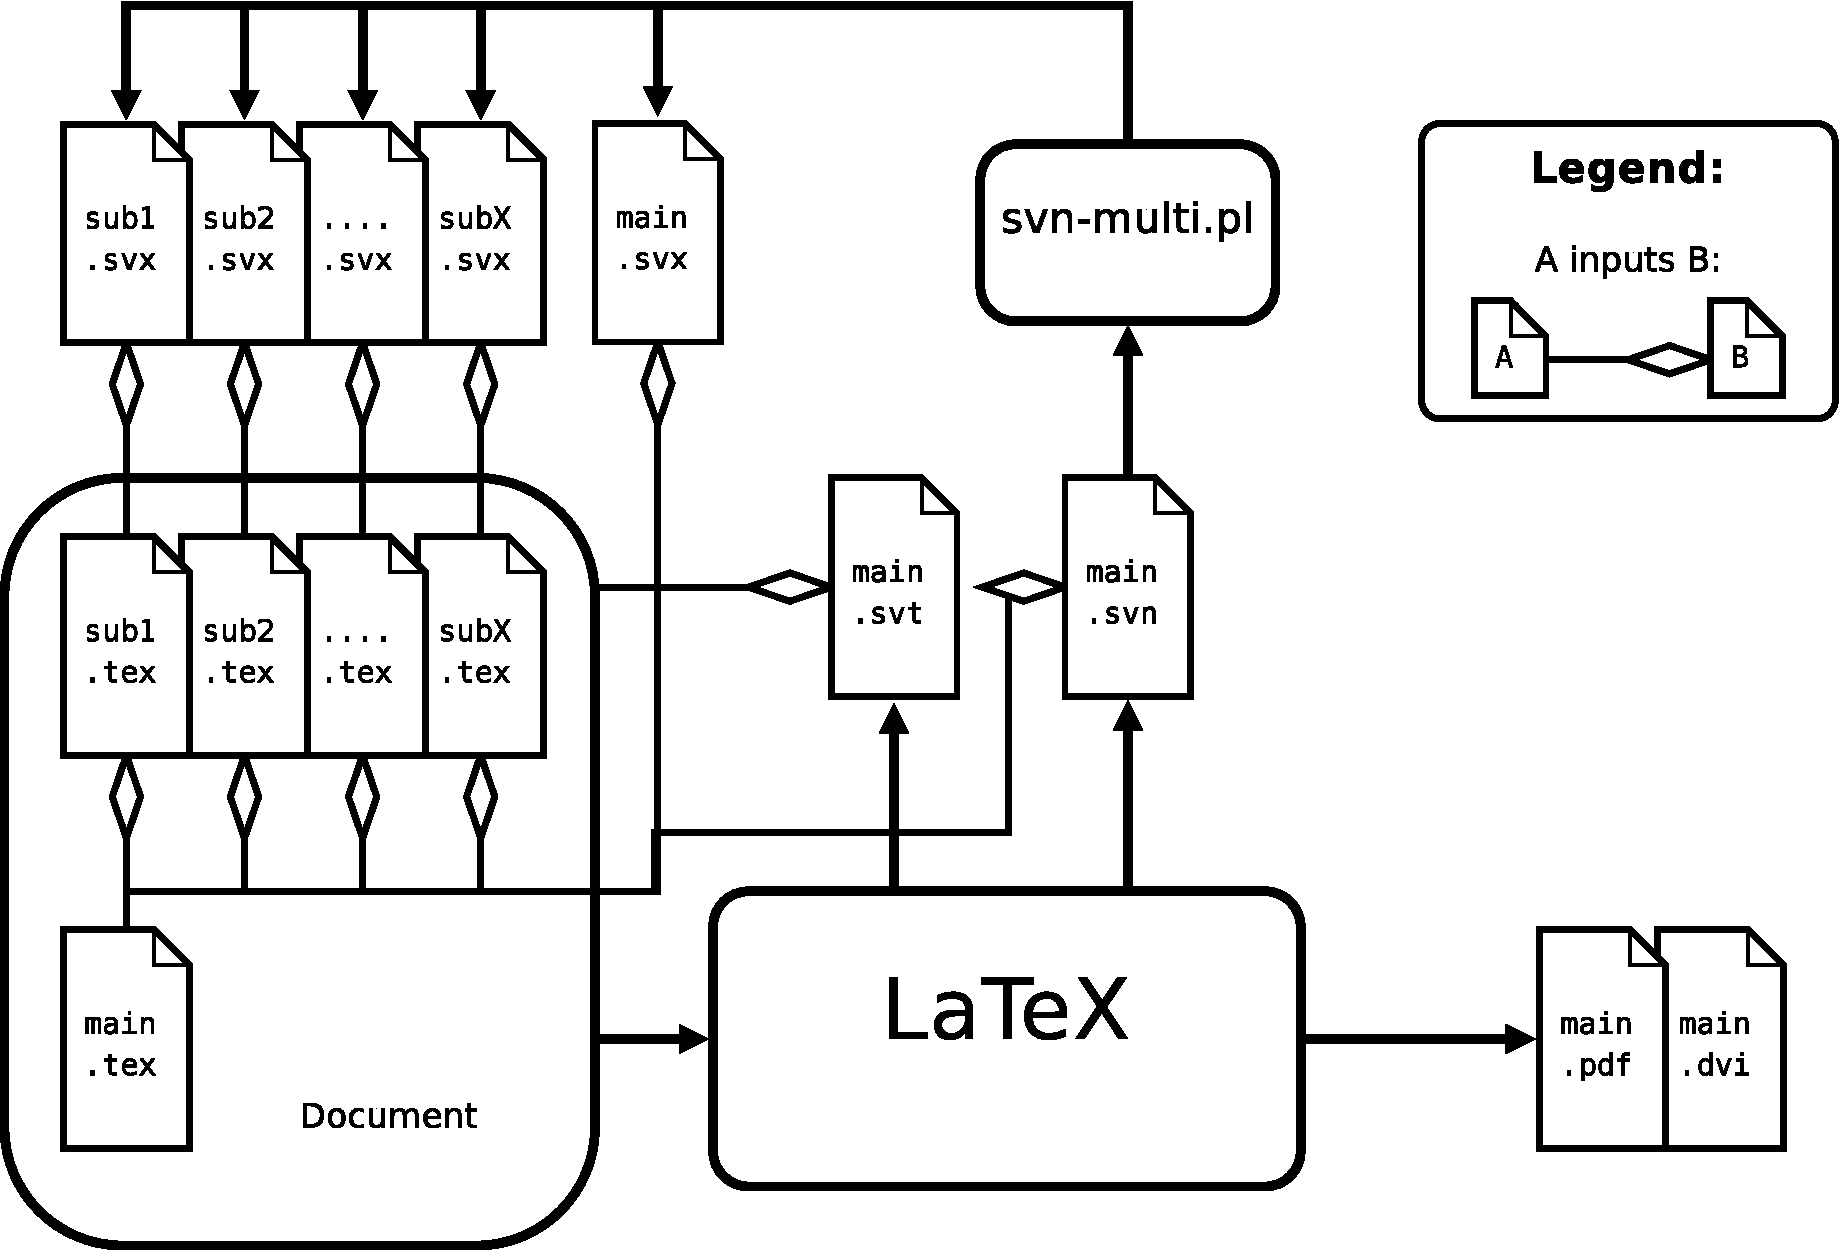
\includegraphics[width=.8\textwidth]{images/compilation.pdf}}
%   \caption{Compilation cycle of documents which use \svnmulti}\label{fig:compi}
% \end{figure}
% \fi
%
% \section{Known Issues}\label{sec:issues}
% This section lists some known issues of the \svnmulti package and tries to
% provide some workaround. Please feel free to write \svnmulti author if you
% detect any side effects or other issues causes by this package.
%
% \subsection{Packet \texttt{listings} uses \cs{input}}
% \textbf{Update:} Newer versions of \svnmulti avoid this issue by changing the catcodes
% back to normal while reading the |.svx| file.
% If a file \meta{basename}.\meta{extension} is typeset verbatim using
% |\lstinputlisting|, which uses |\input| to read the file, an existing
% \meta{basename}|.svx| file is also included as part of the listing. This can
% be avoided by code like this:
% \begin{verbatim}
%  {\makeatletter\let\input\@input
%  \lstinputlisting[options]{filename}
%  }
% \end{verbatim}
%
% \section{Package Dependencies and Acknowledgements}\label{sec:depack}
% This package uses some features from other packages and/or patches some macros
% of them to provide additional related features. This section is used to list
% this packages, their internal macro which got used and acknowledge the
% authors/maintainers of them. Please send error reports to the author of
% \svnmulti and not to the people listed below.\par
% All packages (including \svnmulti) stand under the \LaTeX\ Project Public
% Licence (LPPL) which can be found at
% \hbox{\url{http://www.latex-project.org/lppl/}} and can be freely downloaded
% from the Comprehensive TeX Archive Network (CTAN) at
% \hbox{\url{http://www.ctan.org/}}.
%
% \newenvironment*{DepPackage}[1]{\ignorespaces
% \subsection*{\pkg{#1}}%
% \def\thedeppackage{#1}%
% \def\infoline##1{\par\smallskip\textbf{##1}\hspace{1em}}%
% }
% {\infoline{Location:} CTAN: \url%
% {http://tug.ctan.org/pkg/\thedeppackage}}
%
% Since v2.3 the authors packages \pkg{currfile} and \pkg{filehook} replacing the 
% previous used (and patched) package \pkg{fink}.
%
% \begin{DepPackage}{hyperref}
% The macro \cs{svnnolinkurl} is resembling the \pkg{hyperref} macro
% |\nolinkurl| and uses some its internal macros from the |\url| macro
% definition.
% \infoline{Used internal macros:} |\hyper@normalise|, |\Hurl|
% \infoline{Version used:} 2008/11/18 v6.78m
% \infoline{Licence:} LPPL, any version
% \infoline{Authors/Maintainers:} Sebastian Rahtz, Heiko Oberdiek
% \end{DepPackage}
%
% \begin{DepPackage}{graphics}
% If the \opt{graphics} option is enabled the following macro is patched to
% record the file name and path of the included graphic.
% \infoline{Patched internal macros:} |\Gin@setfile|
% \infoline{Version used:} 2006/02/20 v1.0o
% \infoline{Licence:} LPPL, any version
% \infoline{Author/Maintainer:} David Carlisle, \LaTeX3 Project
% \end{DepPackage}
%
% \begin{DepPackage}{pgf}
% Like the \pkg{graphics} package above a macro of this package is pathed to
% record the file names and paths of included images when the option
% \opt{pgfimages} is enabled. Because this images pre-declares images for later
% use the internal declared `image macros' are patched as well.
% \infoline{Patched internal macros:} |\pgf@declareimage|,
% \hbox{|\pgf@image@|\meta{image name}|!|}
% \infoline{Used internal macros:} |\pgf@filename|, |\pgf@image|
% \infoline{Version used:} 2008/01/15 v2.00
% \infoline{Licence:} LPPL v1.3c and GPL v2
% \infoline{Author\&Maintainer:} Till Tantau
% \end{DepPackage}
%
% \begin{DepPackage}{latex}
% Parts of the macro definitions of the |\tableofcontents| macros from the
% |article| and |book| class of standard \LaTeX\ were used to define a similar
% \csi{tableofrevisions} macro for both this classes and other similar classes.
% \infoline{Version used:} 2005/09/16 v1.4f
% \infoline{Licence:} LPPL v1.3c
% \infoline{Authors/Maintainers:} \LaTeX3 Project
% \end{DepPackage}
%
% \begin{DepPackage}{currfile}
% The file name and path information are taken from the macros of this package.
% It is from the same author and with the same license as \svnmulti\ itself.
% \infoline{Version used:} 2011/01/03 v0.3
% \end{DepPackage}
%
% \begin{DepPackage}{filehook}
% This package is used to install file hooks to update subversion macros for subfiles etc.
% It is from the same author and with the same license as \svnmulti\ itself.
% \infoline{Version used:} 2011/01/03 v0.4
% \end{DepPackage}
%
% \section{Further Reading}
% The \textsf{svn-multi} package (in version 1.3) and its usage got discussed in
% the following articles:
%
% \begin{itemize}
%  \item[{[1]}] Martin Scharrer, ``Version Control of LaTeX Documents with
%  svn-multi'', The Prac\TeX\ Journal, (3), 2007.
%  URL: \url{http://www.tug.org/pracjourn/2007-3/scharrer/}
%  \item[{[2]}] Mark Eli Kalderon, ``LaTeX and Subversion'',
%  The Prac\TeX\ Journal, (3), 2007.
%  URL: \url{http://www.tug.org/pracjourn/2007-3/kalderon-svnmulti/}
%  \item[{[3]}] Uwe Ziegenhagen , ``LaTeX Document Management with Subversion'',
%  The Prac\TeX\ Journal, (3), 2007.
%  URL: \url{http://www.tug.org/pracjourn/2007-3/ziegenhagen/}
% \end{itemize}
%
% \StopEventually{}
% %%%%%%%%%%%%%%%%%%%%%%%%%%%%%%%%%%%%%%%%%%%%%%%%%%%%%%%%%%%%%%%%%%%%%%%%%%%%
% \section{Implementation}
% \iffalse
%<@svn-multi.sty>
% \fi
%
% \iffalse
%<@svnkw.sty>
% \fi
%
% \Finale
\endinput
